
%%% Local Variables: 
%%% mode: latex
%%% TeX-master: t
%%% End: 

\documentclass{article}

% Housekeeping. 
\usepackage{amsmath}
\usepackage{amssymb}
\usepackage{algorithm}
\usepackage{algorithmic}
\usepackage{graphicx}
\graphicspath{{./}{./Figures/}}
\usepackage{listings}

% Some extra house keeping. By myself. Still I want to say Israa is
% beautiful. 
\usepackage{url}
\usepackage{hyperref}


\begin{document}
% Let the hunt begin.

\section{Introduction}
\label{sec:introduction}

Till now, I really could say nothing about that thesis\ldots Almost no
practical stuff is talked and implemented. In this manner, I am here.


\subsection{Normal Distribution}
\label{sec:normal-distribution}

For this part, the original source goes to
\url{http://www.mathworks.com/help/stats/normal-distribution.html}. 
\subsubsection{Definition}
\label{sec:definition}

The normal pdf is
\begin{equation}
  \label{eq:1}
  y=f(x|\mu,\sigma)=\frac{1}{\sigma\sqrt{2\pi}}\exp^{\frac{-{(x-\mu)}^{2}}{2\sigma^{2}}}
\end{equation}

\subsubsection{Background}
\label{sec:background}

The normal distribution is a two-parameter family of curves. The first
parameter, $\mu$, is the mean. The second, $\sigma$, is the standard
deviation. The standard normal distribution (written $\Phi(x)$) sets
$\mu$ to 0 and $\sigma$ to 1. 
\par
$\Phi(x)$ is functionally related to the error function $erf$.
\begin{equation}
  \label{eq:2}
  erf(x)=2\Phi(x\cdot\sqrt{2})-1
\end{equation}
\par
The first use of the normal distribution was as a continuous
approximation to the binomial. 
\par
The usual justification for using the normal distribution for modeling
is the Central Limit Theorem, which states (roughly) that the sum of
independent samples from any distribution with finite mean and
variance converges to the normal distribution as the sample size goes
to infinity. 

\subsubsection{Parameters}
\label{sec:parameters}

To use statistical parameters such as mean and standard deviation
reliably, you need to have a good estimator for them. The maximum
likelihood estimates (MLEs) provide one such estimator. However, an
MLE might be biased, which means that its expected value of the
parameter might not equal the parameter being estimated. For example,
an MLE is biased for estimating the variance of a normal
distribution. An unbiased estimator that is commonly used to estimate
the parameters of the normal distribution is the \emph{minimum
  variance unbiased estimator (MVUE)}. The MVUE has the minimum
variance of all unbiased estimators of a parameter. 
\par
The MVUEs of parameters $\mu$ and $\sigma^{2}$ for the normal
distribution are the sample mean and variance. The sample mean is also
the MLE for $\mu$. The following are two common formulas for the
variance. 
\begin{equation}
  \label{eq:3}
  s^{2}=\frac{1}{n}\sum_{i=1}^{n}{(x_{i}-\bar{x})}^{2}
\end{equation}
\begin{equation}
  \label{eq:4}
  s^{2}=\frac{1}{n-1}\sum_{i=1}^{n}{(x_{i}-\bar{x})}^{2}  
\end{equation}
where $x_{i}=\sum_{i=1}^{n}\frac{x_{i}}{n}$.
\par
Equation \eqref{eq:3} is the maximum likelihood estimator for
$\sigma^{2}$, and \eqref{eq:4} is the MVUE\@.
\par
As an example, suppose you want to estimate the mean, $\mu$, and the
variance, $\sigma^{2}$ of the heights of all fourth grade children in
the United States. The function normfit returns the MVUE for $\mu$,
the square root of the MVUE for $\sigma^{2}$ and confidence intervals
for $\mu$ and $\sigma^{2}$. Here is a playful example modeling the
heights in inches of a randomly chosen fourth grade class. 
\begin{lstlisting}[language=Matlab]
height = normrnd(50,2,30,1);   % Simulate heights.
[mu,s,muci,sci] = normfit(height)
\end{lstlisting}


\section{Multi-Variate Model}
\label{sec:multi-variate-model}





\subsection{Definition}
\label{sec:definition-1}
The probability density function of the \emph{d}-dimensional
multivariate normal distribution is given by 
\begin{equation}
  \label{eq:5}
  y=f(x,\mu,\sum)=\frac{1}{\sqrt{|\sum|2\pi^{d}}}\exp^{-\frac{1}{2}(x-\mu)\sum^{-1}(x-\mu)'}
\end{equation}
where $x$ and $\mu$ are 1-by-$d$ vectors and $\sum$ is a $d$-by-$d$
symmetric positive definite matrix. While it is possible to define the
multivariate normal for singular $\sum$, the density cannot be written
as above. Only random vector generation is supported for the singular
case. Note that while most textbooks define the multivariate normal
with $x$ and $\mu$ oriented as column vectors, for the purposes of
data analysis software, it is more convenient to orient them as row
vectors, and Statistics Toolbox software uses that orientation. 

\subsection{Background}
\label{sec:background-1}

The multivariate normal distribution is a generalization of the
univariate normal to two or more variables. It is a distribution for
random vectors of correlated variables, each element of which has a
univariate normal distribution. In the simplest case, there is no
correlation among variables, and elements of the vectors are
independent univariate normal random variables. 
\par
The multivariate normal distribution is parameterized with a mean
vector, $\mu$, and a covariance matrix, $\sum$. These are analogous to
the mean $\mu$ and variance $\sigma^{2}$ parameters of a univariate
normal distribution. The diagonal elements of $\sum$ contain the
variances for each variable, while the off-diagonal elements of $\sum$
contain the covariances between variables. 
\par
The multivariate normal distribution is often used as a model for
multivariate data, primarily because it is one of the few multivariate
distributions that is tractable to work with. 






\subsection{Examples}
\label{sec:examples}
This example shows the probability density function (pdf) and
cumulative distribution function (cdf) for a bivariate normal
distribution with unequal standard deviations. You can use the
multivariate normal distribution in a higher number of dimensions as
well, although visualization is not easy. 


% \lstset{language=Matlab}
\begin{lstlisting}[language=Matlab]
mu = [0 0];
Sigma = [.25 .3; .3 1];
x1 = -3:.2:3; x2 = -3:.2:3;
[X1,X2] = meshgrid(x1,x2);
F = mvnpdf([X1(:) X2(:)],mu,Sigma);
F = reshape(F,length(x2),length(x1));
surf(x1,x2,F);
caxis([min(F(:))-.5*range(F(:)),max(F(:))]);
axis([-3 3 -3 3 0 .4])
xlabel('x1'); ylabel('x2');
zlabel('Probability Density');
\end{lstlisting}

\begin{figure}[htbp]
  \centering
  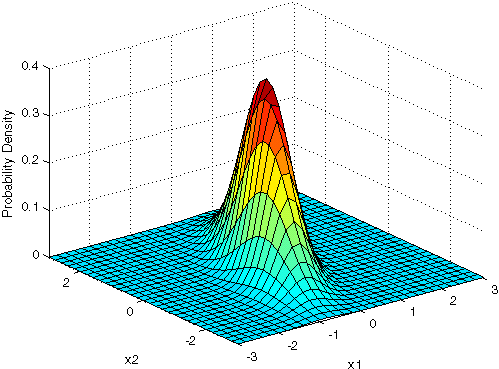
\includegraphics[scale=0.75]{multivariate_normal1}
\end{figure}

\begin{lstlisting}[language=Matlab]
F = mvncdf([X1(:) X2(:)],mu,Sigma);
F = reshape(F,length(x2),length(x1));
surf(x1,x2,F);
caxis([min(F(:))-.5*range(F(:)),max(F(:))]);
axis([-3 3 -3 3 0 1])
xlabel('x1'); ylabel('x2');
zlabel('Cumulative Probability');
\end{lstlisting}

\begin{figure}[htbp]
  \centering
  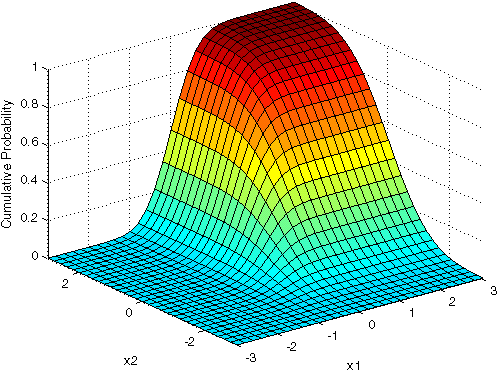
\includegraphics[scale=0.75]{multivariate_normal2}
\end{figure}



\section{e-Quest}
\label{sec:e-quest}

% Just a test for auto-fill mode.
Life is never easy especially when you are living alone in a foreign
country studying computer science. 








\end{document}
